% !TEX root = ../Projektdokumentation.tex
\section{Projektvorbereitung} 
\label{sec:Projektvorbereitung}
Aufgrund des Umfangs des Projekts ging der eigentlichen Projektphase eine Vorbereitungsphase
voraus. Seit Ende November 2014 wurden in regelm\"a\ss{}igen Treffen mit dem Schuldirektor Herrn Hunger 
und ausgew\"ahlten Mitarbeitern die technischen, gestalterischen und inhaltlichen Rahmenanforderungen 
an die neue Homepage festgelegt. Hierbei wurden auch erste Demonstrationsseiten wie
in Abb. \ref{fig:demoSite} erstellt.\\
Die komplette Website w\"ahrend des geplanten Projektblocks fertigzustellen h\"atte m\"oglicherweise
die Einhaltung des Abgabetermins infrage gestellt, weshalb ein wesentlicher Teil der Entwicklung im 
Projektvorfeld stattfand.\\

\begin{figure}[ht]
	
\includegraphics[width=0.9\textwidth]{./Bilder/entwurf_johannes}
	\centering
	\caption{Demonstrationsseite als Diskussionsgrundlage f\"ur das Seitendesign}
	\label{fig:demoSite}
\end{figure}

\subsection{Stand zu Begin der Projektphase}
\label{sec:StandZuBeginDerProjektphase}
Zum Start der Bearbeitungszeit konnten die Autoren auf das von ihnen im Vorfeld entworfene Design 
zur\"uckgreifen. Der allgemeine Aufbau sowie wesentliche Inhalte wurden bereits in den vorausgegangenen 
Meetings festgelegt.\\
Die lokale Entwicklungsumgebung hatten die Autoren vorbereitet und ben\"otigte Software installiert. 
F\"ur die Seite war schon ein funktionsf\"ahiges Basis-Template fertiggestellt. Die Extension zur 
Darstellung der Stundenpl\"ane war zum Gro\ss{}teil fertig entwickelt, jedoch noch nicht in TYPO3 eingebunden.

\subsection{Zielgruppenanalyse}
\label{sec:Zielgruppenanalyse}
Als Zielgruppe der Seite wurden definiert:
\begin{itemize}
	\item{Lehrlinge/Sch\"uler und Lehrer der Schule}
	\item{zuk\"unftige Lehrlinge/Sch\"uler der Schule}
	\item{Partner und Freunde der Schule}
	\item{Mitglieder und Interessenten des F\"ordervereins der Schule}
	\item{Eltern der Lehrlinge/Sch\"uler}
\end{itemize}

\subsection{Designentwurf}
\label{sec:Designentwurf}
Beim Entwerfen des Designs sind mehrere Faktoren mit eingeflossen. Das Hauptaugenmerk
lag hierbei darauf, dass die \"offentliche Wahrnehmung der Medienkompetenz der Schule
stark von der Gestaltung der Internetpr\"asenz abh\"angt.
Die Idee war, mit einem modernen, schlichtem Design die \acs{CI} der Schule zu st\"arken, 
und die Zielgruppe optimal anzusprechen.\\
Zur Verbesserung der \acs{CI} lag also die erste Aufgabe in der Neugestaltung des 
Logos in Verbindung mit dem Banner. Hierbei musste unter anderem darauf 
geachtet werden die Schulfarben passend einflie\ss{}en zu lassen.
Au\ss{}erdem musste zur Darstellung von Neuigkeiten eine passende Form gefunden 
werden.\\
Die gro\ss{}e Herausforderung bestand darin, den Zugang zu vielen Informationen und Materialien 
\"ubersichtlich in einem modernen und \acs{Responsive Design} zu vereinen.Um den Auftraggebern 
eine realistischen Eindruck zu vermitteln ,wurden verschiedene Designentw\"urfe ausgearbeitet 
und mit der Schulleitung und den betreuenden Lehrern diskutiert. Der in Abb. \ref{fig:Grobentwurf} 
dargestellte Seitenentwurf zeigt eine grobe Idee f\"ur die Startseite w\"ahrend der Vorbereitungsphase.

\begin{figure}[ht]
	\centering
	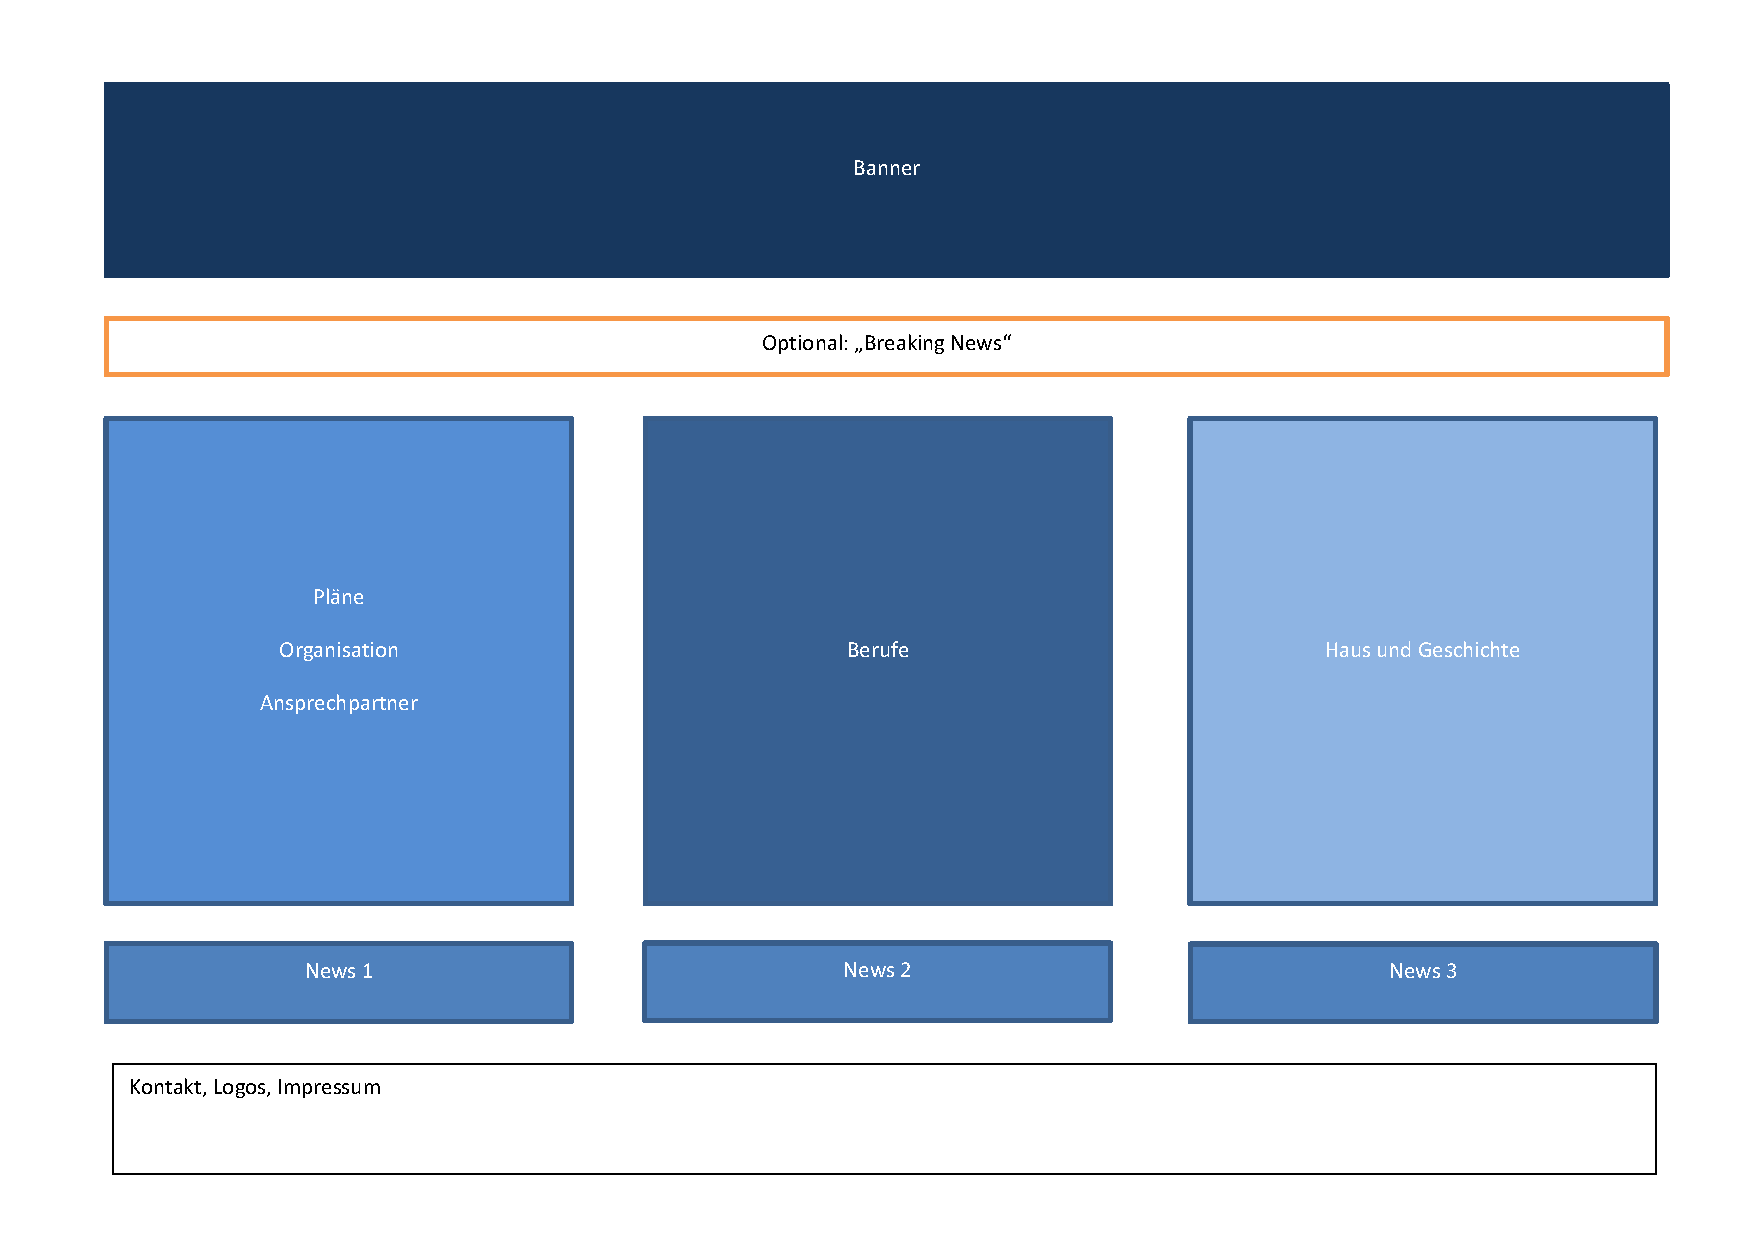
\includegraphics[width=1\textwidth]{./Bilder/Idee_ISC_Startseite}
	\caption{Erster Entwurf der Startseite}
	\label{fig:Grobentwurf}
\end{figure}
\input

\subsection{Zielplattformen}
\label{sec:Zielplattformen}
Selbstverst\"andlich sollten alle g\"angigen Browser (Mozilla Firefox, Internet Explorer, Google 
Chrome, Safari, Opera) im Stande sein, die Seite fehlerfrei darzustellen. Eine optionale 
Zielstellung der Schulleitung war, die Seite \acs{responsive} zu gestalten.

\subsection{Seitenstruktur}
\label{sec:Seitenstruktur}

\begin{figure}[ht]
	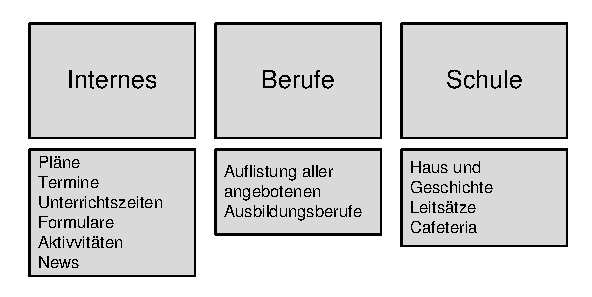
\includegraphics[width=0.50\textwidth]{./Bilder/Menuestruktur}
	\centering
	\caption{Grobe Men\"ustruktur}
	\label{fig:MS}
\end{figure}

 In den vorausgehenden Besprechungen wurden diverse Strukturierungsstrategien eruiert.\\
 In Abb. \ref{fig:MS} ist eine vereinfache Darstellung der geplanten
 Men\"ustrukturierung dargestellt.